\begin{frame}{Fibraciones y Cofibraciones}
En distintos contextos matemáticos encontramos dos problemas básicos, común a todos ellos: el problema de la extensión y el problema del levantamiento. \par
\vspace{1em}
Para estudiar estos problemas, vamos a ver dos conceptos: las fibraciones y las cofibraciones.
\end{frame}


\begin{frame}[fragile]{El problema de la extensión}
Dado un diagrama de aplicaciones continuas 
\[
\begin{tikzcd}
	A \rar{f} \dar[hook, swap]{i} & Y \\
	X \urar[dashed, swap]{\tilde{f}}	&
\end{tikzcd} 
\]
donde $i$ es una inclusión en un contexto dado, ¿cuándo existe $\tilde{f}$ extensión de $f$? 
\end{frame}


%\begin{frame}{El problema de la extensión}
%\begin{teor}[de Extensión de Tietze]
%Sea $X$ normal, $A \subset X$ cerrado, $I \subset \mathbb{R}$ intervalo. Entonces toda $f : A \rightarrow I $ continua admite una extensión $\tilde{f} : X \rightarrow I$ continua.
%\end{teor}
%\pause
%\begin{teor}
%La esfera $S^{n}$ no es un retracto del disco $D^{n+1}$. En otras palabras, la identidad $S^{n} \rightarrow S^{n}$ no se extiende a $D^{n+1}$.
%\end{teor}
%\end{frame}

\begin{frame}[fragile]{Cofibraciones}
\begin{defin}[(Propiedad de extensión homotópica)]
Sea $A \subset X$ un subespacio. Decimos que $i : A \longhookrightarrow X$ o el par $(X, A)$ tiene la \alert{propiedad de extensión homotópica} (HEP) con respecto al espacio $Y$ si dada una homotopía
\[ G : A \times I \longrightarrow Y \]
existe $f: X \longrightarrow Y $ tal que $f(a) = G(a, 0)$ $\forall \ a \in A$, entonces existe $F : X \times I \longrightarrow Y$ tal que $f(x) = F(x,0)$ y $F(a,t) = G(a, t)$ $\forall \ t \in I, \ a \in A$.
\end{defin}
\pause
\begin{defin}
Decimos que un par $(X,A)$ (o la inclusión $i: A \longhookrightarrow X$) es una \alert{cofibración} si posee la HEP con respecto a todo espacio $Y$. \par 
\end{defin}
\end{frame}

%\begin{frame}{Cofibraciones}
%Obsérvese que no toda inclusión es una cofibración. Un contraejemplo es el siguiente:
%\[
%A =  \bigcup_{n \in \bb{N}} \left\lbrace (t, \frac{t}{n}) : t \in [0,1] \right\rbrace \cup \{0\} \times [0,1] \cup [0,1] \times \{0\}
%\]
%\pause
%\begin{tabular}{ll}
%\begin{minipage}{0.5\textwidth}
%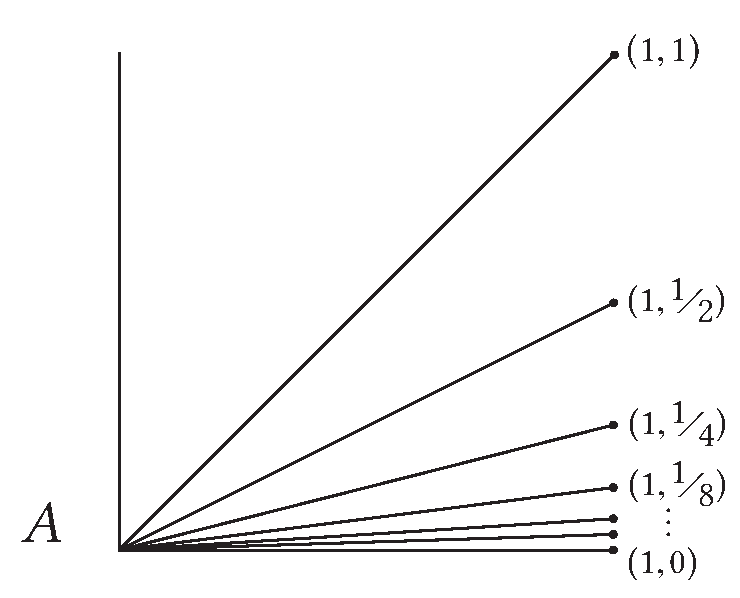
\includegraphics[width=0.8\textwidth]{images/ejcofibsegmentos}
%\end{minipage}
%&
%\begin{minipage}{0.5\textwidth}
%\pause
%El espacio $A$ no es un retracto de $I^2$, por lo tanto, no existe una extensión de la aplicación identidad.
%\end{minipage}
%\end{tabular}
%\end{frame}
%
%\begin{frame}{Cofibraciones}
%\begin{teor}
%Si el par $(X, A)$ es una cofibración y $A$ es contráctil, entonces la aplicación $q : X \longrightarrow \faktor{X}{A}$ es una equivalencia de homotopía.
%\end{teor}
%\pause
%\begin{ejems}
%\begin{enumerate}
%\item Si $G$ es un grafo finito, toda arista con distintos finales se puede contraer a un punto. En este caso, toda componente de $G$ es homótopa o bien a un punto o a una suma puntual de $S^1$. \pause
%\item Consideremos el espacio formado por la unión de una $S^2$ y un segmento por los polos. \par
% Si identificamos los polos al mismo punto sobre la esfera o contraemos el segmento a un punto, obtenemos dos espacios homotópicamente equivalentes. 
%\end{enumerate}
%\end{ejems}
%\end{frame}

\begin{frame}[fragile]{Adjunción de espacios}
\begin{figure}
\centering
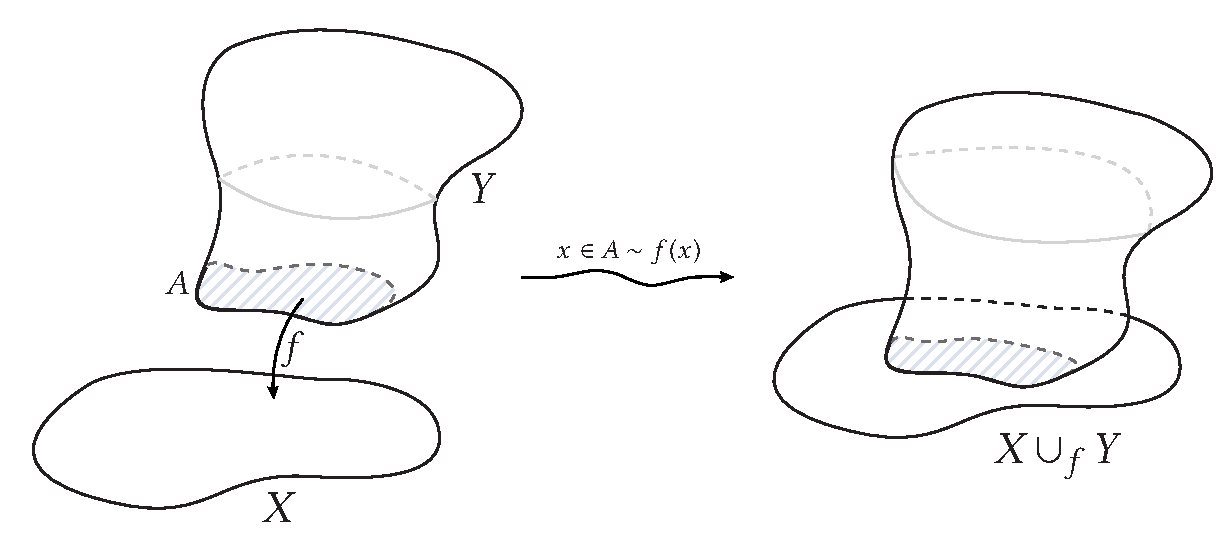
\includegraphics[width = 0.4\textwidth]{images/pegadoespacios}
\end{figure}
Consideramos dos espacios topológicos $X$ e $Y$, un subespacio $A \subset Y$ y una aplicación $f: A \longrightarrow X$. \par
Definimos entonces la adjunción de los dos espacios como
\[ X \cup_f Y := \faktor{X \dot{\cup} Y}{\sim} \ , \qquad \text{donde }x \in A \sim f(x). \]
\end{frame}

\begin{frame}{Cilindro y cono de una aplicación}
\begin{tabular}{ll}
\begin{minipage}{0.5\textwidth}
\centering
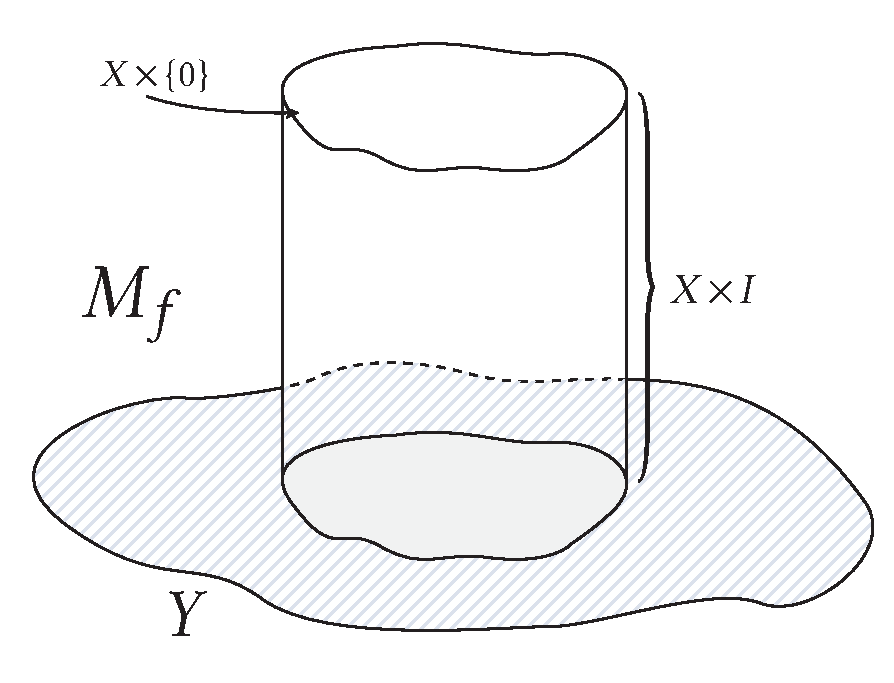
\includegraphics[width = 0.7\textwidth]{images/cilindrof}
\par
El cilindro de una aplicación $f$ se define como:
\[M_f = Y \cup_{\tilde{f}} (X \times I), \] 
\end{minipage}
& \pause
\begin{minipage}{0.5\textwidth}
\centering
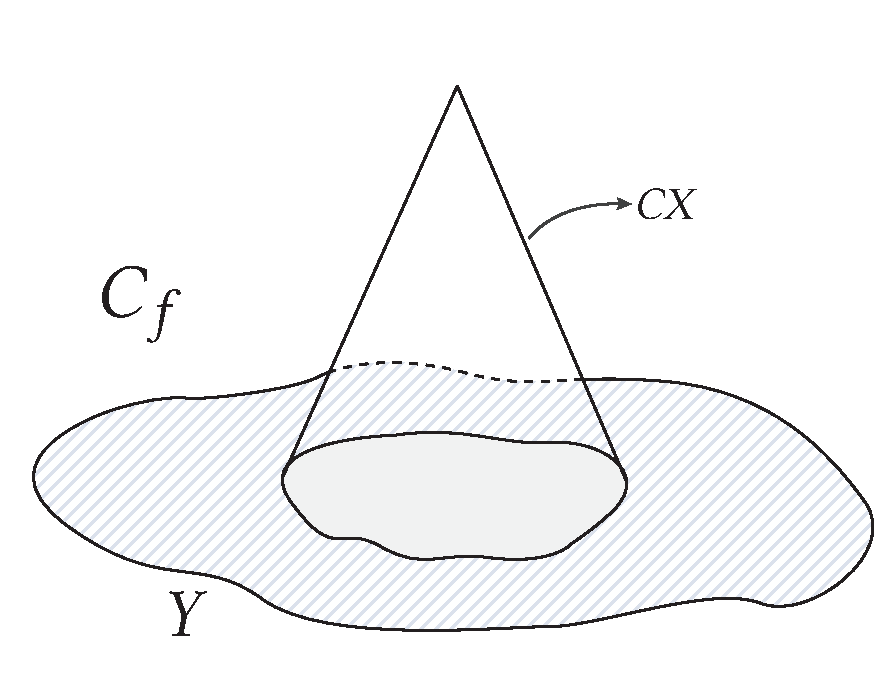
\includegraphics[width = 0.7\textwidth]{images/conof}
\par
El cono de $f$ se define como:
\[ C_f = \faktor{Y \: \dot{\cup} \: CX}{\scriptstyle (x,1) \sim f(x)} \, . \]
\end{minipage}
\end{tabular}
\end{frame}

\begin{frame}{Cofibraciones}
Podemos factorizar la función $f :  X \longrightarrow Y$ como la composición $f = p \circ i$, donde $i$ es la inclusión y $p$ es la aplicación de retracción del cilindro al espacio $Y$.
\pause
\begin{teor}
Sea $f : X \longrightarrow Y$ una aplicación y consideremos la factorización, $f = p \circ i$. Entonces $i$ es una cofibración y $p$ una equivalencia de homotopía. En particular, toda aplicación $f$ puede verse como una cofibración. 
\end{teor}
\end{frame}

%\begin{frame}{Cofibraciones}
%Si tenemos la cofibración $A \longhookrightarrow X$, podemos considerar la sucesión
%\[ A \longhookrightarrow X \longrightarrow \faktor{X}{A} \, .\]
%\pause
%Si $f : X \longrightarrow Y$ es una aplicación cualquiera, tenemos
%\[ X \longrightarrow M_f \longrightarrow \faktor{M_f}{X} = C_f \, , \]
%que podemos escribir como: 
%\[ X \stackrel{f}{\longrightarrow} Y \stackrel{q}{\longrightarrow} C_f \, . \]
%\pause
%De aquí se obtiene la \alert{sucesión de Barratt-Puppe}:
%\[ X \stackrel{f}{\longrightarrow} Y \stackrel{q}{\longrightarrow} C_f \stackrel{\delta}{\longrightarrow} \Sigma X \stackrel{\Sigma f}{\longrightarrow} \Sigma Y \stackrel{\Sigma q}{\longrightarrow} \Sigma C_f \longrightarrow \dots \]
%\end{frame}

\begin{frame}[fragile]{El problema del levantamiento}
El otro problema con el que nos encontramos es el problema del levantamiento de aplicaciones continuas. Dado un diagrama
$$
\begin{tikzcd}
	{}	& X \dar[two heads]{\ p} \\
	Y \urar[dashed]{\tilde{f}} \rar[swap]{f} & B
\end{tikzcd}
$$
donde $p$ es sobreyectiva, ¿cuándo existe $\tilde{f}$ levantamiento de $f$?
\end{frame}

\begin{frame}[fragile]{Fibraciones}
\begin{defin}[(Propiedad de levantamiento homotópico)]
Una aplicación $p : E \longrightarrow B$ tiene la \alert{propiedad de levantamiento homotópico} (HLP) con respecto a un espacio $X$ si dada una homotopía 
\[
G : X \times I \longrightarrow B
\]
existe $g : X \longrightarrow E$ tal que  $G(x, 0) = pg(x)$, existe entonces $\widetilde{G} : X \times I \longrightarrow E$ tal que $\widetilde{G}(x,0) = g(x)$ y $G = p \circ \widetilde{G}$.
\end{defin}
\par \pause
\begin{defin}
Decimos que la aplicación $p : E \longrightarrow B$ es una \alert{fibración} si posee la HLP con respecto a cualquier espacio.
\end{defin}
\end{frame}

\begin{frame}[fragile]{Pullback}
\begin{defin}
Sean $f : X \longrightarrow Z$ y $g: Y \longrightarrow Z$ dos aplicaciones con un codominio común. El pullback de las aplicaciones $f$ y $g$ se define: 
\[P = \{ (x, y) \in X \times Y \ \vert \ f(x) = g(y) \} \subset X \times Y \]
\[
\begin{tikzcd}
P \arrow{rr}{p_Y} \arrow{dd}{p_X} && Y \arrow{dd}{g} \\
\\
X \arrow{rr}{f} && Z
\end{tikzcd}
\]
\end{defin}
\end{frame}

\begin{frame}[fragile]{Fibraciones}
Dada $f: X \longrightarrow Y$ una aplicación cualquiera, podemos descomponerla de la siguiente forma
\[
\begin{tikzcd}
X \arrow{rr}{f} \drar{\varphi} & & Y \\
 & E_f = \{ (x, \omega ) \in X \times Y^I \ \vert \ f(x) = \omega(0) \} \urar[twoheadrightarrow]{p_1} &
\end{tikzcd}
\]
donde $E_f$ es el pullback de $p_1$ y $f$.
\pause
\begin{teor}
Toda aplicación $f : X \longrightarrow Y$ es, salvo homotopía, una fibración. 
\end{teor}
\end{frame}

